\documentclass[10pt]{article}
\usepackage[utf8]{inputenc}
\usepackage{tikz}
\usetikzlibrary{positioning,arrows}
\usetikzlibrary{shapes.geometric}
\tikzstyle{w}=[draw, circle, inner sep=8pt, minimum size=6pt, node distance=2.5cm, fill = lightgray]

\begin{document}
\begin{figure}[h]
	\centering
	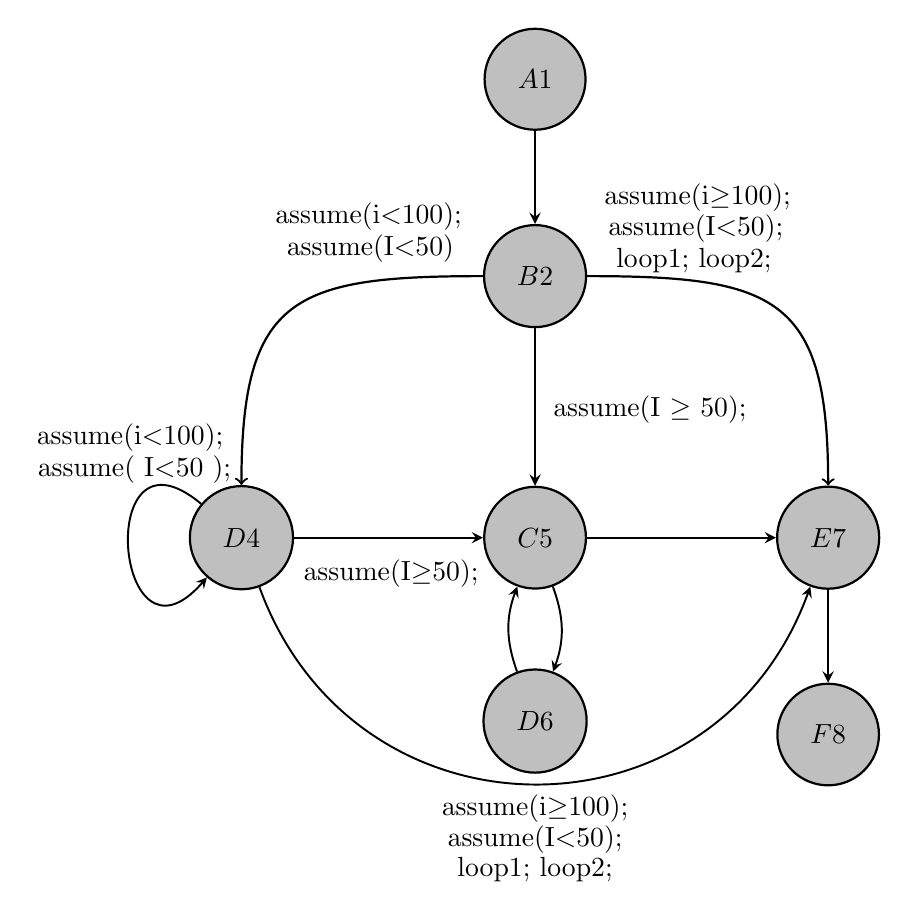
\begin{tikzpicture}[thick]
		\node[w] (A1) at ( 0, 0) {$A1$};
		\node[w] (B2) [below of = A1] {$B2$};
		\node[w] (C5) [below = 2 cm of B2] {$C5$};
		\node[w] (E7) [right = 2.4 cm of C5] {$E7$};
		\node[w] (D4) [left = 2.4 cm of C5] {$D4$};
		\node[w] (F8) [below of = E7] {$F8$};
		\node[w] (D6) [below = 1 cm of C5] {$D6$};
		\draw (A1) edge[->,>=stealth] (B2) node[right, xshift=7.5mm, yshift=-15mm] {assume(i$\geq$100);} node[right, xshift=8mm, yshift=-19mm] {assume(I$<$50);} node[right, xshift=9mm, yshift=-23mm] {loop1; loop2;};
		\draw (B2) edge[->,>=stealth] (C5) node[right, xshift=+1mm, yshift=-17mm] {assume(I $\geq$ 50);} node[left, xshift=-9mm, yshift=+3.5mm] {assume(I$<$50)} node[left, xshift=-8mm, yshift=+7.5mm] {assume(i$<$100);};
		\draw (C5) edge[->,>=stealth] (E7);
		\draw (D4) edge[->,>=stealth] (C5) node[below, xshift=+19mm, yshift=-1.5mm] {assume(I$\geq$50);};
		\draw (E7) edge[->,>=stealth] (F8);
		\draw (C5) edge[->,>=stealth,bend left=20, line width=.7pt] (D6);
		\draw (D6) edge[->,>=stealth,bend left=20, line width=.7pt] (C5) node[below, yshift=-8mm] {assume(i$\geq$100);} node[below, yshift=-12mm] {assume(I$<$50);} node[below, yshift=-16mm] {loop1; loop2;};
		\draw (D4) edge[->,>=stealth,out=140,in=229,looseness=4.9, line width=.7pt] (D4);
		\draw[->] (B2.east) .. controls +(right:2.4cm) and +(up:2.4cm) .. (E7.north);
		\draw[->] (B2.west) .. controls +(left:2.4cm) and +(up:2.4cm) .. (D4.north) node[left, yshift=+2mm] {assume( I$<$50 );} node[left, xshift=-1mm, yshift=+6mm] {assume(i$<$100);};
		\draw (D4) edge[->,>=stealth,out=-70,in=250,looseness=1.3, line width=.7pt] (E7);
	\end{tikzpicture}
  \label{fig:sat-reduction-edges}
\end{figure}
\end{document}
